\documentclass[12pt, a4paper]{article}

\usepackage{listings}
\usepackage{color}
\usepackage{enumitem}
\usepackage{amsthm}
\usepackage{amssymb}
\usepackage{listings}
\usepackage{setspace}
\usepackage{graphicx}
\graphicspath{ {./figures/} }


\title{Deep Learning Fundamentals}
\author{William Darko}
\date{Summer 2021}

\pagenumbering{arabic}

\begin{document}

\maketitle
\newpage

\tableofcontents

\newpage

\section{About this course}
\paragraph*{}
Explore deep learning from scratch or broaden understanding of deep learning, via
practical hands-on code examples to solve concrete problems. We'll
utilise the Python language, and deep learning framework Keras with Tensor flow as a backend engine



\newpage

\section{Resources}

\begin{itemize}
   \item \textbf{Deep Learning with Python} (1st Edition) by François Chollet.
   Manning publisher
\end{itemize}

\newpage

\section{What is deep learning?}

\subsection{Artificial Intelligence}
{
   \centering
   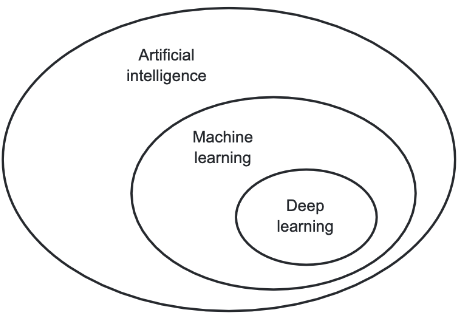
\includegraphics[width=8cm]{AI_Umbrella.png}

   the umbrella of Artificial intelligence

}

\paragraph*{}
We'll define Artificial intelligence to be the \textit{effort to automate intellectual 
tasks normally performed by humans.} AI is the general field that encompasses machine learning,
which deep learning is a subfield of.

Early AI took the approach of programmers manually implementing a large set of 
rules for manupulating knowledge; this was known as \textbf{symbolic AI}.

Symbolic AI turned out intractable, when applied to more complex problems like
image classification, speech recogition, language translation, etc.

Machine Learning was the new AI paradigm that rose to replace symbolic AI.
\end{document}